
Aqui el alumno debe describir su proceso de trabajo, como se trabajo, problemas, lo que funciono, pruebas de tecnologias ...

\section{Diseño de arquitectura}

Especificar la decisión relacionada respecto a servidores de datos y aplicación (web)
\begin{itemize}
    \item Servidores propios,
    \item Hosting, 
    \item Cloud, otros o mezcla de ellos.
\end{itemize}
Incluya un esquema que represente la integración de estos elementos, desde el punto de vista físico y lógico. Este diagrama debe ser explicado. Por ejemplo: 
Tal como se representa en la Ilustración 2 la arq. que da soporte al  sw “mi software” se divide en 2 servidores físicos, ATLANTA y MARCUS. 
EL primero aloja el server web sobre un SO apache xxx, para el sw mio.midominio.cl http://146.83.99.99, puerto ssh 999 u puerto apache 999. El segundo  servidor físico aloja 2 componentes lógicos, servidor de archivos user/carpeta/ y de base de datos con Mysql 192.168.l.0 (ejemplo). Los usuarios locales acceden a través de los sistemas distribuidos por red local y al sistema web vía internet…. etc.
El escenario es distinto si se trabaja con contenedores, si se utilizan servicios web, API, o la nube amazon ws, azure, etc

\begin{figure}[H]
    \centering
    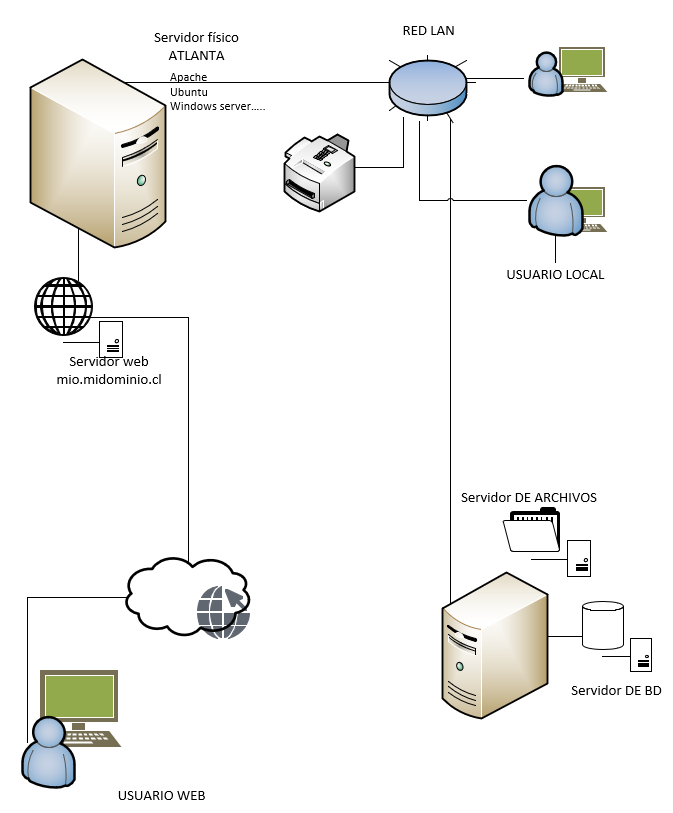
\includegraphics[scale=0.5]{figures/i6.png}
    \caption{Ejemplo2}
    \label{fig:e6}
\end{figure}


\section{Estructura del código}

Si se utiliza framework o se programa en lenguaje web puro indicar la forma como se organizan físicamente los archivos y si estos respetan alguna arquitectura de programación como modelo vista controlador, o 3 capas, etc. Incluya una imagen del árbol de directorio.

\subsection{Backend}

 \begin{table}[H]
    \begin{center}
        \begin{tabular}{ | m{2cm} | m{8cm} | }
            \hline \textbf{Directorio} & \textbf{Detalle }\\ \hline
            Controllers & Funciones con las que cuenta la aplicación al momento de comunicarse con el servidor de base de datos y viceversa.   \\ \hline
                &    \\ \hline    
                &    \\ \hline   
              \end{tabular}
        \caption{E2}
    \end{center}
\end{table}


Funcionalidad- Endpoints a utilizar:
\begin{enumerate}
    \item 1. http://”URLPROYECTO”.cl/”RUTA A UTILIZAR”
    \begin{enumerate}
        \item a. Tipo de petición:
            \begin{itemize}
               \item i. “get,post,put,delete”
            \end{itemize}
        \item b. Parámetros a ingresar, el tipo de datos y restricciones
            \begin{enumerate}
                \item i. Nombre
                    \begin{enumerate}
                        \item 1. String
                        \item 2. Requerido
                        \item 3. Tamaño mínimo de 1 caracteres
                        \item 4. Tamaño máximo de 100 caracteres
                    \end{enumerate}
                \item  ii. Precio
                    \begin{enumerate}
                        \item 1. Number
                        \item 2. No requerido - Default 10
                    \end{enumerate}
            \end{enumerate}
    \end{enumerate}
    \item 2. http://”URLPROYECTO”.cl/”RUTA A UTILIZAR”
        \begin{enumerate}
            \item a. Tipo de petición:
                \begin{enumerate}
                    \item i. “get,post,put,delete”
                \end{enumerate}
            \item b. Parámetros a ingresar, el tipo de datos y restricciones
        \begin{enumerate}
            \item i. Nombre
                \begin{enumerate}
                    \item 1. String
                    \item 2. Requerido
                    \item 3. Tamaño mínimo de 1 caracteres
                    \item 4. Tamaño máximo de 100 caracteres
                \end{enumerate}
            \item  ii. Precio
                \begin{enumerate}
                    \item 1. Number
                    \item 2. No requerido - Default 10
                \end{enumerate}
           \end{enumerate}
    \end{enumerate}    
\end{enumerate}

\subsection{Frontend}

 \begin{table}[H]
    \begin{center}
        \begin{tabular}{ | m{2cm} | m{8cm} | }
            \hline \textbf{Directorio} & \textbf{Detalle }\\ \hline
             &    \\ \hline
            &    \\ \hline    
            &    \\ \hline   
        \end{tabular}
        \caption{E2}
    \end{center}
\end{table}